% Dieser Text ist urheberrechtlich gesch\"utzt
% Er stellt einen Auszug eines von mir erstellten Referates da
% und darf nicht gewerblich genutzt werden
% die private bzw. Studiums bezogen Nutzung ist frei
% April 2011
% Autor: Sascha Frank 
% Universit\"at Freiburg 
% www.informatik.uni-freiburg.de/~frank/
% frank < was da sonst immer steht > tf.uni-freiburg.de

\documentclass[hyperref={pdfpagelabels=false}, 12pt]{beamer}
% Die Hyperref Option hyperref={pdfpagelabels=false} verhindert die Warnung:
% Package hyperref Warning: Option `pdfpagelabels' is turned off
% (hyperref)                because \thepage is undefined. 
% Hyperref stopped early 
%

%neue Rechtschreibung
\usepackage[ngerman]{babel}
\usepackage{babelbib}
 
%\usepackage[T1]{fontenc}
%Umlaute ermölichen utf8 ( latin1)
\usepackage[utf8]{inputenc}

\usepackage{hyperref}
\usepackage{graphicx}
\usepackage{lmodern}

% Pseudocode in latex
\usepackage{algorithm2e}
\usepackage{tikz}


% Das Paket lmodern erspart die folgenden Warnungen:
% LaTeX Font Warning: Font shape `OT1/cmss/m/n' in size <4> not available
% (Font)              size <5> substituted on input line 22.
% LaTeX Font Warning: Size substitutions with differences
% (Font)              up to 1.0pt have occurred.
%

% Wenn \titel{\ldots} \author{\ldots} erst nach \begin{document} kommen,
% kommt folgende Warnung:
% Package hyperref Warning: Option `pdfauthor' has already been used,
% (hyperref) ... 
% Daher steht es hier vor \begin{document}


\title{Verkehrsflusssimulation einer Kreuzung durch ein angepasstes Nagel-Schreckenberg-Modell }  
\author{ Julian Berndt, Hannah Dusch, Martin Kraus, Philipp Schwarz} 
\date{\today} 
%\titlegraphic{\includegraphics[width=8cm]{steintuermchen} }
% zusaetzlich ist das usepackage{beamerthemeshadow} eingebunden 
\usepackage{beamerthemeshadow}

%  \beamersetuncovermixins{\opaqueness<1>{25}}{\opaqueness<2->{15}}
%  sorgt dafuer das die Elemente die erst noch (zukuenftig) kommen 
%  nur schwach angedeutet erscheinen 
\beamersetuncovermixins{\opaqueness<1>{25}}{\opaqueness<2->{15}}
% klappt auch bei Tabellen, wenn teTeX verwendet wird\ldots
 \pdfcompresslevel=9 
\begin{document}
{
%\setbeamertemplate{frametitle}[default][center]
%\setbeamertemplate{background canvas}
\begin{titlepage}

\end{titlepage}

\begin{frame}
\frametitle{Inhaltsverzeichnis}
\tableofcontents
\end{frame} 

\section{Aufgabenstellung}
\begin{frame}
	\frametitle{Aufgabenstellung}
	\begin{itemize}
		\item Zwei einspurige Ringstraßen
		\item Nur in einer Richtung befahrbar (Einbahnstraßen)
		\item Straße wird nicht verlassen
		\item Kreuzung in einem Punkt, mit Rechts-Vor-Links
		\item Verkehrsdichten getrennt einstellbar
	\end{itemize}
\end{frame}

\section{Modellierung}
\begin{frame}
	\frametitle{Nagel-Schreckenberg}
	\begin{algorithm}[H]
 %\SetLine % For v3.9
 %\SetAlgoLined % For previous releases [?]
 \KwData{ \\
   \(v_{i}, v_{max}, d(i,j), p \) 
 }
 \KwResult{ \\
    Update für Fahrzeug $i$
 }

 %initialization\;
 \For{ \(i \in \{1, \cdots, n\}\) }{
   Beschleunigen: \(v_{i} := min\{ v_{i}+1,v_{max}\} \);
   \\Bremsen: \(v_{i} := d(i,i+1), \text{ falls } v_{i} > d(i,i+1) \);
   \\Trödeln: \(v_{i} := max\{(v_{i}-1, 0 \}  \text{ mit } p < 1 \);
   \\Bewegen: Fahrzeug $i$ um \(v_{i}\) Zellen vorwärts bewegen;
 }
 
 \label{algo:nagelsberg}
\end{algorithm}

\end{frame}

\begin{frame}
	\frametitle{Erweitertes Modell }
	\begin{itemize}
		\item Vor der Kreuzung werden die Autos abgebremst
		\item Abbiegen nicht möglich
		\item Kreuzung jeweils auf der Mitte der Straße
		\item Autos auf der vertikalen Straße haben Vorfahrt
	\end{itemize}
\end{frame}

\section{Simulationsprogramm}
\begin{frame}
	\frametitle{Programmbedienung}
	%
	hier kommt das Programm...
	%
\end{frame}

\begin{frame}
	\frametitle{Implementierung}
Straßen:
\begin{itemize}
  \item Anzahl der Zellen \(N \in \mathbb{N}\)
  \item Anzahl der Zeitschritte, die Simuliert werden \(T \in \mathbb{N}\)
  \item Koordinate des Kreuzungspunktes \(c \in \{ 1, \ldots N \}\)
\end{itemize}
Fahrzeuge:
\begin{itemize}
  \item Autonummer \(k \in \{ 1, \ldots, K \}, \; K \leq N\) 
  \item Geschwindigkeit \(v_k \in \{0, \ldots, v_{max} \}\)
  \item Position, d.h. Straße und Zellenkoordinate
\end{itemize}
\end{frame}

\begin{frame}
	\frametitle{Implementierung}
	Daher zwei $T\times N$-Matrizen $V,$ $W$ und ganzzahliges $c$ mit 
	\begin{itemize}
		\item $t$-te Zeile ist Straße zum Zeitpunkt $t$
		\item $n$-te Spalte ist die $n$-te Zelle 
		\item $V=$ Geschwindigkeitsmatrix, $W=$ Autonummermatrix
		\item $c$ ist die Position der Kreuzungszelle
	\end{itemize}
	Beispiel: 
	\[
  V = 
  \begin{bmatrix}
    v_1& 0& 0& v_2& v_3 \\
    0& 0& 0& 0& 0
  \end{bmatrix}, \;
  W = 
  \begin{bmatrix}
    1& 0& 0& 2& 3 \\
    0& 0& 0& 0& 0
  \end{bmatrix}, \;
  c = 3
\]
	
\end{frame}

\section{Validierung}

\begin{frame}
	\frametitle{Fundamentaldiagramm}
	Dazu:
	\begin{itemize}
		\item Verkehrsdichte $\rho=\frac{\#\text{Autos}}{\#\text{Zellen}}$
		\item Verkehrsfluss $f = \frac{P}{\delta T}$ \\
	mit $P$ Anzahl der Autos, die den Messpunkt während $\delta T$ passieren
	\end{itemize}
	
	\begin{figure}[H]%
		\centering
		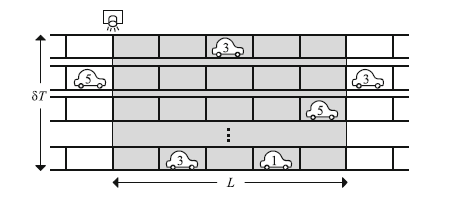
\includegraphics[width=6cm]{4_BestFD.png}%
	\end{figure}
\end{frame}

\begin{frame}
	\frametitle{Vergleich Einzelstraße ohne Kreuzung}
		\begin{figure}[H]%
		\centering
		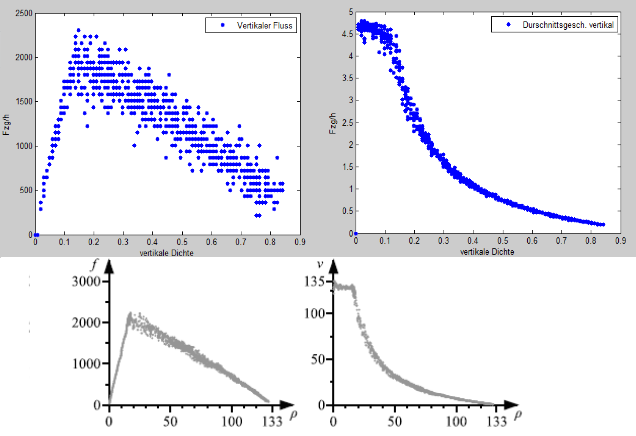
\includegraphics[height=6cm]{4_FD_Vergleich.png}%
	\end{figure}
\end{frame}

\begin{frame}
	\frametitle{Zellen-Zeit-Diagramm}
		\begin{figure}[H]%
		\centering
		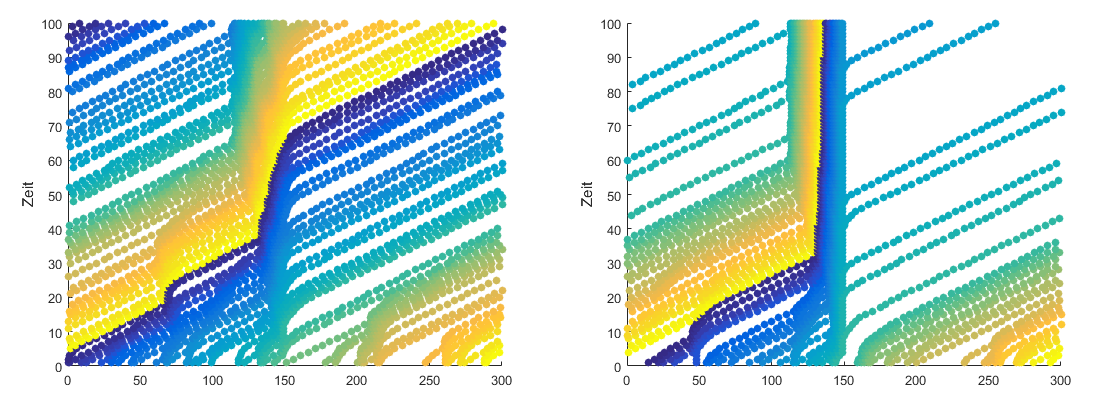
\includegraphics[width=11cm]{4_ZelleZeit.png}
		\caption{Links: vertikale Straße, Rechts: horizontale Straße}
	\end{figure}
	\tiny{vertikale Dichte $\rho_v=0.11$,\\ horizontale Dichte $\rho_h =0.12$,\\ Trödelwkeit $p=0.2$}
	
\end{frame}

\section{Fazit}
\begin{frame}
	\frametitle{Verkehrsfluss Kreuzung}
	\begin{figure}[H]%
		\centering
		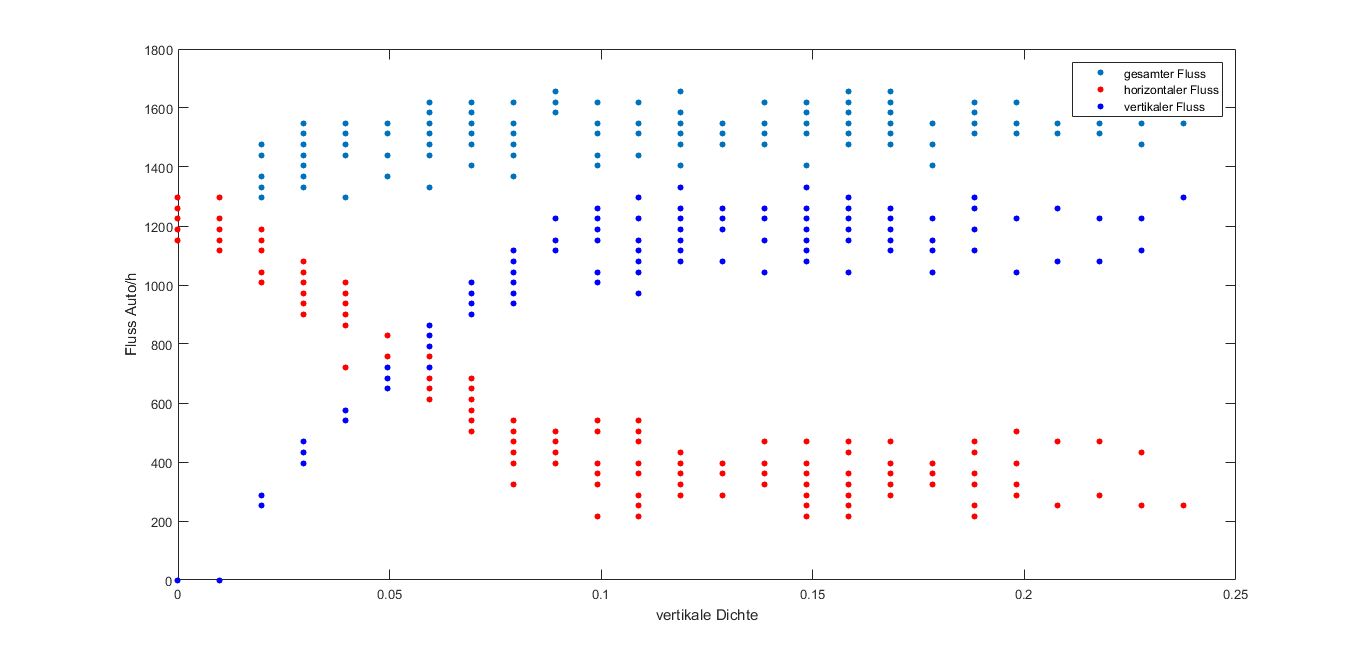
\includegraphics[width=11cm]{MaxFluss.png}
	\end{figure}
	\tiny{horizontale Dichte $\rho_h =0.12$,\\ Trödelwkeit $p=0.2$}
\end{frame}


\end{document}